\documentclass[10pt,a4paper]{article}
\usepackage[margin=2.2cm]{geometry}
\usepackage{fontspec}
\usepackage{kotex}
\setmainfont{Apple SD Gothic Neo}
\setsansfont{Apple SD Gothic Neo}
\usepackage{amsmath,amssymb}
\usepackage{graphicx}
\usepackage{caption}
\usepackage[dvipsnames]{xcolor}
\usepackage[colorlinks=true,linkcolor=MidnightBlue,citecolor=MidnightBlue,
            urlcolor=MidnightBlue]{hyperref}
\usepackage{titlesec}
\titleformat{\section}{\large\bfseries}{\thesection}{0.6em}{}
\captionsetup{font=small,labelfont=bf}
\setlength{\parskip}{0.35em}
\setlength{\parindent}{0pt}
\usepackage{mdframed}
\newmdenv[linewidth=0.4pt,linecolor=gray!60,backgroundcolor=gray!5,
          innertopmargin=6pt,innerbottommargin=6pt,skipabove=8pt,skipbelow=8pt]{claimbox}
\newcommand{\claim}[2]{\begin{claimbox}\textbf{주장.} #1\par\smallskip
  \textcolor{gray!70}{\textbf{반증 조건.} #2}\end{claimbox}}

\title{\bfseries 이름의 해로움은 `틀린 이름'의 해로움이었다\\[2pt]
\large 무정체 자의 일반화 --- 그리고 KR 창($n^{\dagger}{=}10$)은 이중 인공물}
\author{월드모델 실험실 · 노트 $853$}
\date{2026-08-09}
\begin{document}\maketitle

\section{한 줄}

$852$ 의 `이름을 지우면 강해진다'가 $n{=}1$ 짝 위에 있다는 티처 \#$18$ 적발의
이행. 같은 $12$씨앗 적합 한 벌에서 앱·CN 을 $4$팔로 재니 --- \textbf{앱은
격차가 정확히 $0.0000$}(모바일-정체 $=$ 무정체 $0.3123$ · 원핫이 평가 $189$행
순위를 전혀 안 바꾼다), CN 은 $+0.0351$(평가 $19$행 --- 참고 수준), KR 은
$+0.1358$. \textbf{정련된 법칙: 이름의 해로움 $=$ 이름이 틀렸을 때다} --- KR
만화에 `JP 만화' 이름은 $-0.136$, 비게임 앱에 `모바일' 이름은 같은 모집단이라
$0$. \textbf{무정체는 어느 짝에서도 해롭지 않았다 $\to$ 서빙 기본값 승격
(약우위).}

\begin{figure}[t]\centering
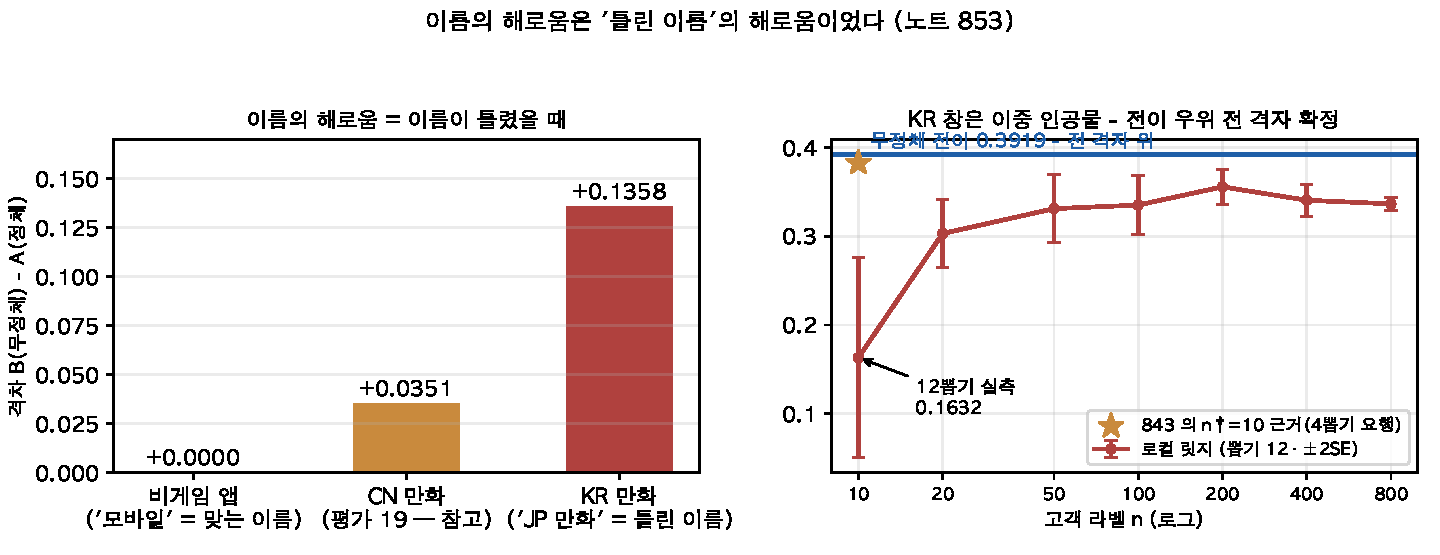
\includegraphics[width=0.97\textwidth]{figs/wrongname.pdf}
\caption{왼쪽: 세 짝의 격차 --- 틀린 이름일수록 크다. 오른쪽: KR 릿지
재판정($12$뽑기 · $\alpha$ 단일 · 지문 일치) --- 전 격자가 전이 아래.}
\end{figure}

\claim{\textbf{KR 의 `창'($843$ 의 $n^{\dagger}{=}10$)은 이중 인공물이었다.}
릿지 곡선을 뽑기 $12$ · $\alpha{=}1$ 단일 · 라벨 지문 대조로 다시 재니
$n{=}10$ 은 $0.3826$ 이 아니라 \textbf{$0.1632$}($4$뽑기 요행이 $+0.22$ 를
만들었다), 최고점은 $n{=}200$ 의 $0.356$ --- $+2$SE 를 얹어도 무정체 전이
$0.3919$ 아래다. \textbf{KR 는 라벨 $800$건까지도 전이가 왕이다.} 앱은
반대로 로컬 조기 우위가 산다(전이 $0.312$ 는 경로 무관 · 릿지 $n800$
$0.503$ · 창 $n^{\dagger} \approx 20{\sim}50$). $822$ 의 `도메인마다 다르다'가
무정체 자 위에서 서빙 정책이 됐다: \textbf{이득 지도가 곧 라우팅 표다 ---
만화류는 전이 · 앱은 일찍 로컬.}}
{CN 은 평가 $19$행이라 부호만 기록(표본이 자라면 재판정). 앱의 `정확히 $0$'
은 순위 보존적 원핫의 실측 사례 --- 예측 벡터 대조는 재현 러너로 가능.
기제(JP 눈금 대 KR)는 걸지 않는다 --- 예측 채점 $3/4$(앱 격차 $\ge 0.05$
미스 · 순서·문턱 적중대 유지).}

\section{정직}

$852$ 정직 문장 정정: `B 의 강함이 OOC\_DROP 보정 덕인지 미분해'는 틀림 ---
보정은 죽은 코드다(티처 \#$18$ 실측 · 호출자 $0$). A/B 차는 코드상
\textbf{원핫 $12$칸 단독}. 논문 $203$ 의 `H$1$ 확정'은 `$d0$ 에서 H$2$ 기각 ·
타 뽑기 미검' 병기로 강등. 서빙 지뢰 등록: names 미등록 이름 predict 는
\texttt{\_feat} 의 ALL$5$ 폴백이 $36$열을 조용히 오정렬 --- 규약화 전 서빙
금지. GitHub 흐름 $13$회째. 판 $\rho$ $0.4710$ 그대로.

\end{document}
